\documentclass[12pt]{article}
\parindent0pt
\usepackage{ctex}
\usepackage{amsmath}
\usepackage{mathtools,amssymb}
\usepackage{tikz}
\title{assignemnt 5}
\author{Longyu Zhu}
\begin{document}
\section*{10.1}
\subsection*{Exercise 4}
this graph has undirected edges, and no loop\\
so this graph is a multigraph\\
\\
\subsection*{Exercise 6}
this graph has undirected edges, and no loop\\
so this graph is a multigraph\\
\\
\subsection*{Exercise 8}
this graph has directed edges,and it have loop\\
so that graph is a directed multigraph\\
\\
\subsection*{Exercise 12}
R={(u,v)} \\
let $(b,a)\in R $ first ,because that is undirected so wecan get an edge (b,a)$\in R$ that shown R is symmetric.\\
and $(a,a)\in R$ is also available for this graph, so that is reflexive\\
so R is summetric and reflexive\\
\\
\subsection*{Exercise 24}
three calls from 555-0011 to 555-8888\\
two calls from 555-8888 to 555-0011\\
two calls from 555-2222 to 555-0091\\
two calls from 555-1221 to each other number\\
one call from 555-1333 to 555-0011\\
one call from 555-1333 to 555-1221\\
one call from 555-1333 to 555-1200\\


\tikzset{every picture/.style={line width=0.75pt}} 
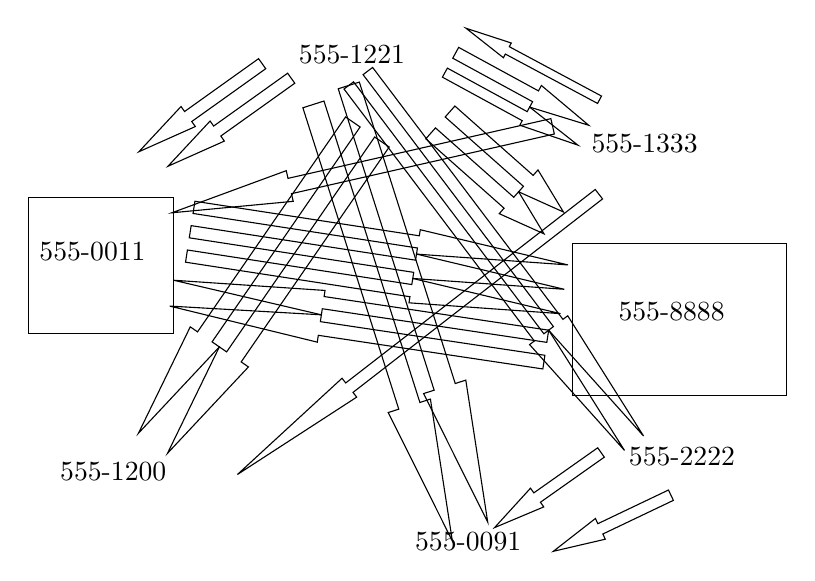
\begin{tikzpicture}[x=0.75pt,y=0.75pt,yscale=-1,xscale=1]
\draw   (81.16,74.6) -- (101.47,52.81) -- (103.19,55.22) -- (138.83,29.76) -- (142.28,34.59) -- (106.64,60.04) -- (108.36,62.46) -- cycle ;
\draw   (92.35,103.2) -- (200.47,119.84) -- (200.92,116.91) -- (272.1,133.87) -- (199.12,128.65) -- (199.57,125.71) -- (91.45,109.07) -- cycle ;
\draw   (90.55,114.94) -- (198.66,131.58) -- (199.12,128.65) -- (270.29,145.61) -- (197.31,140.38) -- (197.76,137.45) -- (89.64,120.81) -- cycle ;
\draw   (94.16,91.46) -- (202.28,108.1) -- (202.73,105.17) -- (273.9,122.13) -- (200.92,116.91) -- (201.37,113.97) -- (93.26,97.33) -- cycle ;
\draw   (263.71,159.44) -- (155.53,143.24) -- (155.09,146.17) -- (83.85,129.5) -- (156.85,134.43) -- (156.41,137.36) -- (264.59,153.57) -- cycle ;
\draw   (261.79,172.25) -- (153.61,156.04) -- (153.12,159.33) -- (81.98,141.95) -- (155.09,146.17) -- (154.6,149.46) -- (262.78,165.67) -- cycle ;
\draw   (13.85,89.5) -- (83.85,89.5) -- (83.85,155) -- (13.85,155) -- cycle ;
\draw   (276,112) -- (379,112) -- (379,185) -- (276,185) -- cycle ;
\draw   (291.41,214.74) -- (260.64,236.47) -- (262.23,238.72) -- (238.53,248.69) -- (255.85,229.69) -- (257.45,231.95) -- (288.22,210.23) -- cycle ;
\draw   (324.69,235.56) -- (290.69,251.78) -- (291.88,254.28) -- (266.84,260.11) -- (287.12,244.3) -- (288.31,246.8) -- (322.31,230.58) -- cycle ;
\draw   (67.16,67.6) -- (87.47,45.81) -- (89.19,48.22) -- (124.83,22.76) -- (128.28,27.59) -- (92.64,53.04) -- (94.36,55.46) -- cycle ;
\draw   (283.9,54.85) -- (255.43,46.09) -- (256.85,43.49) -- (218.39,22.53) -- (221.23,17.32) -- (259.68,38.28) -- (261.1,35.68) -- cycle ;
\draw   (278.69,64.42) -- (250.68,54.81) -- (251.86,52.63) -- (213.41,31.67) -- (215.79,27.31) -- (254.24,48.27) -- (255.43,46.09) -- cycle ;
\draw   (271.7,96.62) -- (250.12,86.9) -- (252.45,84.26) -- (214.74,50.84) -- (219.41,45.57) -- (257.12,78.99) -- (259.45,76.36) -- cycle ;
\draw   (262.36,107.16) -- (240.78,97.43) -- (243.11,94.8) -- (205.4,61.38) -- (210.07,56.11) -- (247.78,89.53) -- (250.12,86.9) -- cycle ;
\draw   (66.94,203.24) -- (91.92,151.96) -- (95.42,154.38) -- (166.74,50.84) -- (173.75,55.67) -- (102.43,159.2) -- (105.94,161.62) -- cycle ;
\draw   (80.95,212.89) -- (105.94,161.62) -- (109.44,164.03) -- (180.76,60.5) -- (187.77,65.32) -- (116.45,168.86) -- (119.95,171.27) -- cycle ;
\draw   (235.23,246.02) -- (204.33,184.11) -- (209.42,182.49) -- (163.21,37.27) -- (173.38,34.04) -- (219.58,179.26) -- (224.67,177.64) -- cycle ;
\draw   (218.2,255.16) -- (187.3,193.25) -- (192.38,191.63) -- (146.18,46.41) -- (156.34,43.17) -- (202.55,188.39) -- (207.63,186.78) -- cycle ;
\draw   (301.14,211.5) -- (255.4,160.51) -- (257.7,158.78) -- (166,37.39) -- (170.59,33.92) -- (262.29,155.31) -- (264.59,153.57) -- cycle ;
\draw   (310.32,204.56) -- (264.59,153.57) -- (266.89,151.84) -- (175.18,30.45) -- (179.78,26.98) -- (271.48,148.37) -- (273.78,146.63) -- cycle ;
\draw   (83.03,97.01) -- (138.17,76.72) -- (139.01,80.42) -- (265.66,51.66) -- (267.33,59.05) -- (140.68,87.8) -- (141.52,91.49) -- cycle ;
\draw   (224.76,8.09) -- (246.58,15.21) -- (245.63,16.99) -- (290.05,40.77) -- (288.15,44.32) -- (243.73,20.53) -- (242.79,22.3) -- cycle ;
\draw   (114.64,223.1) -- (165.04,176.73) -- (166.81,179) -- (287.03,85.78) -- (290.56,90.33) -- (170.33,183.55) -- (172.1,185.83) -- cycle ;
\draw (18,110) node [anchor=north west][inner sep=0.75pt]   [align=left] {555-0011};
\draw (143,15) node [anchor=north west][inner sep=0.75pt]   [align=left] {555-1221};
\draw (284,58) node [anchor=north west][inner sep=0.75pt]   [align=left] {555-1333};
\draw (297,139) node [anchor=north west][inner sep=0.75pt]   [align=left] {555-8888};
\draw (302,209) node [anchor=north west][inner sep=0.75pt]   [align=left] {555-2222};
\draw (199,250) node [anchor=north west][inner sep=0.75pt]   [align=left] {555-0091};
\draw (28,216) node [anchor=north west][inner sep=0.75pt]   [align=left] {555-1200};
\end{tikzpicture}
\\
\section*{10.2}
\subsection*{Exercise 4}
the sum=2 * number of edges\\
a)\\
deg(a)=2,deg(b)=4,deg(c)=1,deg(d)=0,deg(e)=2,deg(f)=3\\
so the sum is 6*2=12\\
\\
b)\\
deg(a)=4+2(loop)=6,deg(b)=6,deg(c)=4+2(loop)=6,deg(d)=5,deg(e)=3\\
so the sum is 2*13=26\\
\\
c)\\
deg(a)=3,deg(b)=2,deg(c)=4,deg(d)=0,deg(e)=6,deg(g)=4,deg(h)=2,deg(i)=3,deg(f)=0\\
so the sum is 2*12=24\\
\\
\subsection*{Exercise 10}
the sum of the in = the sum of the out = the number of egdes of the graph.\\
a)\\
in(a)=3,out(a)=1\\
in(b)=1,out(b)=2\\
in(c)=2,out(c)=1\\
in(d)=1,out(d)=3\\
in(sum)=7,out(sum)=7\\
so the number of edges of the graph=7\\
\\
b)\\
in(a)=2,out(a)=2\\
in(b)=3,out(b)=4\\
in(c)=2,out(c)=1\\
in(d)=1,out(d)=1\\
in(sum)=8,out(sum)=8\\
so the number of edges of the graph=8\\
\\
c)\\
in(a)=6,out(a)=1\\
in(b)=1,out(b)=5\\
in(c)=2,out(c)=5\\
in(d)=4,out(d)=2\\
in(e)=0,out(e)=0\\
in(sum)=13,out(sum)=13\\
so the number of edges of the graph=13\\
\\
\subsection*{Exercise 26}
$K_n$ n=1 and n=2\\
$C_n$ n be the even number\\
$W_n$ no values n\\
$Q_n$ all number bigger than 2\\
\\
\subsection*{Exercise 28}
a)\\
$V_1$={Zamora,Agraharam,Smith,Chou.Macintyre}\\
$V_2$={Planning,Publicity,Sales,Marketing,Development,Industry relations}\\
E={(Zamora,Planning),(Zamora,Sales),(Zamora,Marketing),(Zamora,Industry relations),(Agraharam,Planning),
(Agraharam,Development),(Smith,Sales),(Smith,Publicity),(Smith,Industry relations),(Chou,sales),(Chou,Publicity)
(Chou,Industry relations),(Macintyre,Planning),(Macintyre,Sales),(Macintyre,Publicity),(Macintyre,Industry relations)}\\
\\
b)\\
Zamora-Marketing\\
Agraharam-Development\\
Smith-Publicity\\
Chou-Sales\\
Macintyre-Planning\\
but the match can be vary\\
\\
c)\\
the answer of (b) is the complete matching, and max matching\\
becasue the complete matching always be the max matching\\
\\
\section*{10.3}
\subsection*{Exercise 6}
$$
\left[
\begin{matrix}
    0 & 1 & 0 & 1 & 0\\
    1 & 0 & 0 & 1 & 1\\
    0 & 0 & 0 & 1 & 1\\
    1 & 1 & 1 & 0 & 0\\
    0 & 1 & 1 & 0 & 0\\
\end{matrix}
\right]
$$
\subsection*{Exercise 8}
$$
\left[
\begin{matrix}
    0 & 1 & 0 & 1 & 0\\
    1 & 0 & 1 & 1 & 1\\
    0 & 1 & 1 & 0 & 0\\
    1 & 0 & 0 & 0 & 1\\
    0 & 0 & 1 & 0 & 1\\
\end{matrix}
\right]
$$
\subsection*{Exercise 10}
\tikzset{every picture/.style={line width=0.75pt}} 
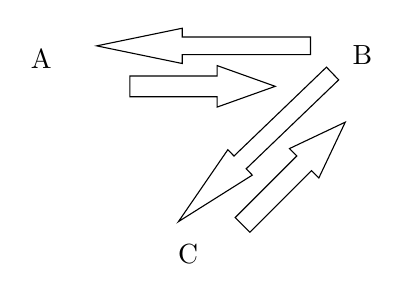
\begin{tikzpicture}[x=0.75pt,y=0.75pt,yscale=-1,xscale=1]
\draw   (88,70) -- (130,70) -- (130,65) -- (158,75) -- (130,85) -- (130,80) -- (88,80) -- cycle ;
\draw   (72,55.5) -- (113.2,47) -- (113.2,51.25) -- (175,51.25) -- (175,59.75) -- (113.2,59.75) -- (113.2,64) -- cycle ;
\draw   (111.37,140.18) -- (135.18,105.51) -- (138.13,108.57) -- (182.69,65.75) -- (188.58,71.88) -- (144.02,114.7) -- (146.96,117.77) -- cycle ;
\draw   (138.72,138.21) -- (168.41,108.51) -- (164.88,104.98) -- (191.75,92.25) -- (179.02,119.12) -- (175.49,115.59) -- (145.79,145.28) -- cycle ;
\draw (39,56) node [anchor=north west][inner sep=0.75pt]   [align=left] {A};
\draw (194,54) node [anchor=north west][inner sep=0.75pt]   [align=left] {B};
\draw (110,150) node [anchor=north west][inner sep=0.75pt]   [align=left] {C};
\end{tikzpicture}
\\
\subsection*{Exercise 12}


\tikzset{every picture/.style={line width=0.75pt}} 
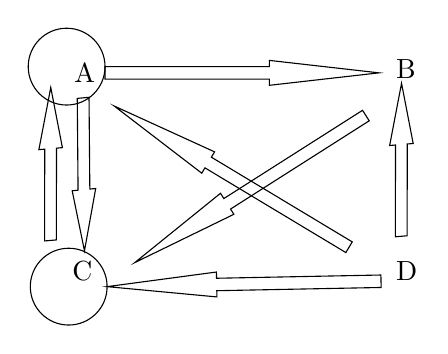
\begin{tikzpicture}[x=0.75pt,y=0.75pt,yscale=-1,xscale=1]
\draw   (18,58.5) .. controls (18,48.28) and (26.28,40) .. (36.5,40) .. controls (46.72,40) and (55,48.28) .. (55,58.5) .. controls (55,68.72) and (46.72,77) .. (36.5,77) .. controls (26.28,77) and (18,68.72) .. (18,58.5) -- cycle ;
\draw   (19,164.5) .. controls (19,154.28) and (27.28,146) .. (37.5,146) .. controls (47.72,146) and (56,154.28) .. (56,164.5) .. controls (56,174.72) and (47.72,183) .. (37.5,183) .. controls (27.28,183) and (19,174.72) .. (19,164.5) -- cycle ;
\draw   (55,58.5) -- (134.2,58.5) -- (134.2,55.5) -- (187,61.5) -- (134.2,67.5) -- (134.2,64.5) -- (55,64.5) -- cycle ;
\draw   (41.63,73.81) -- (42.01,118.03) -- (39.18,118.31) -- (45.1,147.24) -- (50.51,117.21) -- (47.68,117.49) -- (47.29,73.27) -- cycle ;
\draw   (31.54,142) -- (31.63,97.78) -- (34.47,97.53) -- (28.86,68.54) -- (23.13,98.51) -- (25.96,98.26) -- (25.87,142.48) -- cycle ;
\draw   (182.29,84.6) -- (115.47,127.12) -- (117.08,129.65) -- (69.32,152.93) -- (110.64,119.52) -- (112.25,122.06) -- (179.07,79.54) -- cycle ;
\draw   (171.02,148.08) -- (103.14,107.27) -- (101.6,109.84) -- (59.44,77.49) -- (107.78,99.56) -- (106.23,102.13) -- (174.11,142.94) -- cycle ;
\draw   (188.03,164.9) -- (108.85,166.46) -- (108.91,169.46) -- (56,164.5) -- (108.67,157.46) -- (108.73,160.46) -- (187.92,158.9) -- cycle ;
\draw   (200.54,140) -- (200.63,95.78) -- (203.47,95.53) -- (197.86,66.54) -- (192.13,96.51) -- (194.96,96.26) -- (194.87,140.48) -- cycle ;
\draw (39,56) node [anchor=north west][inner sep=0.75pt]   [align=left] {A};
\draw (194,54) node [anchor=north west][inner sep=0.75pt]   [align=left] {B};
\draw (38,151) node [anchor=north west][inner sep=0.75pt]   [align=left] {C};
\draw (194,151) node [anchor=north west][inner sep=0.75pt]   [align=left] {D};
\end{tikzpicture}
\\
\subsection*{Exercise 26}
a)\\
number of edges= 5, the vertices number=6\\
so that is $\frac{5*2}{6*5}=\frac{10}{30}=\frac{1}{3}$\\
\\
b)\\
number of edges= 24, the vertices number=16\\
so that is $\frac{2*24}{16*15}=\frac{48}{240}=\frac{1}{5}$\\
\\
c)\\
number of edges=12 , the vertices number=8\\
so that is $\frac{12*2}{8*7}=\frac{24}{56}=\frac{3}{7}$\\
\\
\end{document}